\documentclass[twoside,11pt]{report}

%%%%%%%%%%%%%%%%%%%%%%%%
\usepackage[english]{babel}
\usepackage[utf8]{inputenc}
\usepackage[top=2.5cm, bottom=2.5cm, left=4.0cm, right=2.5cm]{geometry}
\usepackage{fancyhdr}
\pagestyle{fancy}
\usepackage{amsmath}
\usepackage{listings}
\usepackage{graphicx}
\usepackage{xspace}
%\usepackage[colorinlistoftodos]{todonotes}
\usepackage[nottoc]{tocbibind}
\usepackage{appendix}
\usepackage{slashed}
\usepackage{braket}
%\usepackage{color, soul}
%\usepackage{units}
\usepackage{xcolor}
\usepackage{subcaption}
\usepackage{float}
\usepackage{setspace}
\usepackage[acronym]{glossaries}
\usepackage{appendix}
%\usepackage{utils/tikz-feynman}
\usepackage{feynmp-auto}
\usepackage{comment}
\usepackage{lscape}
\usepackage{placeins}
\usepackage{url}
\usepackage{tikz}
\usepackage{cite}
\usepackage{lineno}
\usepackage[%  
colorlinks=false,
pdfborder={0 0 0},
linkcolor=blue
]{hyperref}
\makeglossaries
%%%%%%%%%%%%%%%%%%%%%%%%
\numberwithin{equation}{section}
\newcommand{\HRule}{\rule{\linewidth}{0.5mm}}
\renewcommand{\arraystretch}{1.25}
\onehalfspacing
%%%%%%%%%%%%%%%%%%%%%%%%
\begin{document}
	\pagenumbering{roman}
	\fancyhead{}
	% latex

\newcommand{\changefont}{\fontsize{9}{11}\selectfont}

% general

\newcommand{\Lagr}{\mathcal{L}}
\newcommand{\ifb}{$\textrm{fb}^{-1}\;$}

% variables

\newcommand{\pt}{$\ensuremath{p_\mathrm{T}}\;$}
\newcommand{\abseta}{$\ensuremath{|\eta |}\;$}
\newcommand{\met}{$E_{\mathrm{T}}^\textrm{miss}\;$}
\newcommand{\mct}{\ensuremath{m_\mathrm{CT}}}
\newcommand{\mt}{\ensuremath{m_\mathrm{T}}}
\newcommand{\mbb}{\ensuremath{m_\mathrm{bb}}}
\newcommand{\drbonebtwo}{\ensuremath{\Delta R (\mathrm{b_1}, \mathrm{b_2})}}
\newcommand{\amttwo}{\ensuremath{am_{\mathrm{T2}}}}
\newcommand{\mwhad}{\ensuremath{m_{\mathrm{W}}^{\mathrm{had}}}}
\newcommand{\bjettwopt}{\ensuremath{p_{\mathrm{T}}\left(b2\right)}}
\newcommand{\mblone}{\ensuremath{m (\ell, \textrm{b}_1)}}
\newcommand{\mbltwo}{\ensuremath{m (\ell, \textrm{b}_2)}}

% sm processes

\newcommand{\ttbar}{\ensuremath{t\bar{t}\,}}
\newcommand{\Wt}{\ensuremath{\mathrm{Wt}}}
\newcommand{\ttV}{\ensuremath{\mathrm{t\bar{t}V}}}
\newcommand{\Wjets}{\ensuremath{\mathrm{W+\textrm{jets}}}}
\newcommand{\Zjets}{\ensuremath{\mathrm{Z+\textrm{jets}}}}
\newcommand{\Wh}{\ensuremath{Wh}\xspace}
\newcommand{\bbbar}{\ensuremath{b\bar{b}}\xspace}


% susy

\newcommand{\oneLbb}{\ensuremath{1 \ell \bbbar}\xspace}
\newcommand{\chargino}{\ensuremath{\tilde{\chi}_{1}^{\pm}}}
\newcommand{\neutralino}{\ensuremath{\tilde{\chi}_{2}^{0}}}
\newcommand{\lsp}{\ensuremath{\tilde{\chi}_{1}^{0}}}
\newcommand{\finalstate}{\ensuremath{\chargino \neutralino \rightarrow W^{\pm}h \lsp \lsp \rightarrow 1\ell^{\pm} + b \bar{b} + E_T^{miss}}}
\newcommand{\SRlbbLow}     {SR1Lbb-Low\xspace}
\newcommand{\SRlbbMedium}  {SR1Lbb-Medium\xspace}
\newcommand{\SRlbbHigh}    {SR1Lbb-High\xspace}

% mc


\newcommand*{\MADGRAPHV}[1]{\textsc{MadGraph}~#1\xspace}
\newcommand*{\MGMCatNLO}{\textsc{MadGraph5}\_aMC@NLO\xspace} 
\newcommand*{\MGMCatNLOV}[1]{\textsc{MadGraph5}\_aMC@NLO~#1\xspace} 
\newcommand*{\POWHEG}{\textsc{Powheg}\xspace}
\newcommand*{\POWHEGV}[1]{\textsc{Powheg}~#1\xspace}
\newcommand*{\POWHEGBOX}{\textsc{Powheg-Box}\xspace}
\newcommand*{\POWHEGBOXV}[1]{\textsc{Powheg-Box}~#1\xspace}
\newcommand*{\POWPYTHIA}{\POWHEG{}+\PYTHIA}
\newcommand*{\PYTHIA}{\textsc{Pythia}\xspace}
\newcommand*{\PYTHIAV}[1]{\textsc{Pythia}~#1\xspace}
\newcommand*{\SHERPA}{\textsc{Sherpa}\xspace}
\newcommand*{\SHERPAV}[1]{\textsc{Sherpa}~#1\xspace}




	% Detector Chapter
\newacronym{lhc}{LHC}{Large Hadron Collider}
\newacronym{cern}{CERN}{European Organisation for Nuclear Research}
\newacronym{ps}{PS}{Proton Synchrotron}
\newacronym{psb}{PSB}{Proton Synchrotron Booster}
\newacronym{sps}{SPS}{Super Proton Synchrotron}
% Randos
\newacronym{sm}{SM}{Standard Model}
\newacronym{bsm}{BSM}{Beyond the Standard Model}
\newacronym{lhc}{LHC}{Large Hadron Collider}
\newacronym{susy}{SUSY}{Supersymmetry}
\newacronym{dm}{DM}{Dark Matter}
\newacronym{hllhc}{HL-LHC}{High-Luminosity LHC}
\newacronym{itk}{ITk}{Inner Tracker}
\newacronym{2hdm}{2HDM}{Two Higgs Doublet model}
\newacronym{ls3}{LS3}{Long Shutdown 3}
\newacronym{bdt}{BDT}{Boosted Decision Tree}
\newacronym{dnn}{DNN}{Deep Neural Network}
\newacronym{mc}{MC}{Monte Carlo}
\newacronym{pv}{PV}{Primary Vertex}

	\def\pythia{\textsc{Pythia8}\xspace}
\def\pythiasix{\textsc{Pythia6}\xspace}
\def\sherpa{\textsc{Sherpa}\xspace} 
\def\alpgen{\textsc{Alpgen}\xspace} 
\def\herwig{\textsc{Herwig}\xspace} 
\def\herwigseven{\textsc{Herwig7}\xspace} 
\def\jimmy{\textsc{JIMMY}\xspace} 
\def\menlops{\textsc{MENLOPS}\xspace} 
\def\mepsatnlo{\textsc{MEPS@NLO}\xspace} 
\def\mepsatlo{\textsc{MEPS@LO}\xspace} 
\def\nloewvirt{NLO~\ensuremath{\text{EW}_\text{virt}}\xspace}
\def\mcatnlo{\textsc{MC@NLO}\xspace} 
\def\mcfm{\textsc{MCFM}\xspace} 
\def\mgamc{\textsc{MadGraph5}\_a\textsc{MC@NLO}\xspace}
\def\mg{\textsc{MadGraph}\xspace}
\def\mgpythia{\textsc{MadGraph5}\_a\textsc{MC@NLO}\ensuremath{+}\pythia}
\def\ggtwovv{\textsc{gg2VV}\xspace} 
\def\vbfnlo{\textsc{VBFNLO}\xspace} 
\def\openloops{\textsc{OpenLoops}\,1\xspace}
\def\openloopstwo{\textsc{OpenLoops}\,2\xspace}
\def\sherpaopenloops{\textsc{Sherpa+OpenLoops}\xspace}
\def\collier{\textsc{Collier}\xspace}
\def\minlo{\textsc{Powheg} MiNLO\xspace}
\def\powhegpythia{\textsc{Powheg}\ensuremath{+}\pythia}
\def\photospp{\textsc{Photos++}\xspace}
\def\minntchannels{\texttt{Min\_N\_TChannels}\xspace}
\def\fxfx{\textsc{FxFx}\xspace}
\def\gosam{\textsc{GoSam}\xspace}
% tunes and PDF sets
\def\cteq{\texttt{CTEQ6L1}\xspace}
\def\ctten{\texttt{CT10}\xspace}
\def\cttennlo{\texttt{CT10nlo}\xspace}
\def\ctfourteennlo{\texttt{CT14nnlo}\xspace}
\def\ctfourteennnlo{\texttt{CT14nnlo}\xspace}
\def\nnpdfonenlo{\texttt{NNPDF3.1nlo}\xspace}
\def\nnpdfnnlo{\texttt{NNPDF3.0nnlo}\xspace}
\def\nnpdfnlo{\texttt{NNPDF3.0nlo}\xspace}
\def\nnpdflo{\texttt{NNPDF3.0lo}\xspace}
\def\nnpdftwo{\texttt{NNPDF2.3lo}\xspace}
\def\nnpdftwonlo{\texttt{NNPDF2.3nlo}\xspace}
\def\mstw{\texttt{MSTW2008nlo}\xspace}
\def\mstwnnlo{\texttt{MSTW2008nnlo}\xspace}
\def\powheg{\textsc{Powheg}\xspace}
\def\powhegbox{\textsc{PowhegBox}\xspace}
\def\powhegboxRes{\textsc{PowhegBoxRes}\xspace}
\def\powhegboxpythia{\textsc{PowhegBox}\ensuremath{+}\pythia}
\def\powhegboxRespythia{\textsc{PowhegBoxRes}\ensuremath{+}\pythia}
\def\vbfnlopythia{\textsc{VBFNLO}\ensuremath{+}\pythia} 
\def\powhegboxherwig{\textsc{PowhegBox}\ensuremath{+}\herwig} 
\def\powhegboxherwigseven{\textsc{PowhegBox}\ensuremath{+}\herwigseven} 
\def\amcpeight{\mgamc+\pythia}
\def\mcatnloherwig{\textsc{MC@NLO}\ensuremath{+}\herwig} 
\def\madspin{\textsc{MadSpin}\xspace}
\def\photos{\textsc{Photos}\xspace} 
\def\photospp{\textsc{Photos++}\xspace}
\def\evtgen{\textsc{EvtGen}\xspace}
\def\hathor{\textsc{Hathor}\xspace} 
\def\aFourTeen{\texttt{A14}\xspace}
\def\auet{\texttt{AUET2}\xspace}
\def\aznlo{\texttt{AZNLO}\xspace}
\def\mmhtnnlo{\texttt{MMHT2014nnlo}\xspace}
\def\mmhtnlo{\texttt{MMHT2014nlo}\xspace}
\def\mmhtlo{\texttt{MMHT2014lo}\xspace}
\def\ueee{\texttt{UE-EE-5}\xspace}
\def\Gmu{\ensuremath{G_{\mu}}\xspace}
\def\hdamp{\ensuremath{h_{\mathrm{damp}}}\xspace}
\def\ttbar{\ensuremath{t\bar{t}}\xspace}
\def\ttHF{\ensuremath{t\bar{t}}+HF\xspace}

\def\hdamp{\ensuremath{h_{\mathrm{damp}}}\xspace}
\def\mtop{\ensuremath{m_{\mathrm{top}}}\xspace}
\def\mur{\ensuremath{\mu_\mathrm{r}}\xspace}
\def\muf{\ensuremath{\mu_\mathrm{f}}\xspace}
\def\muq{\ensuremath{\mu_\mathrm{q}}\xspace}

\def\ttH{\ensuremath{t\bar{t}H}\xspace}
\def\ttV{\ensuremath{t\bar{t}V}\xspace}
\def\ttW{\ensuremath{t\bar{t}W}\xspace}
\def\ttZ{\ensuremath{t\bar{t}Z}\xspace}
\def\ttZnunu{\ensuremath{t\bar{t}Z(\to\nu\nu)}\xspace}
\def\ttZqq{\ensuremath{t\bar{t}Z(\to qq)}\xspace}
\def\ttee{\ensuremath{t\bar{t}e^+e^-}\xspace}
\def\ttmumu{\ensuremath{t\bar{t}\mu^+\mu^-}\xspace}
\def\tttautau{\ensuremath{t\bar{t}\tau^+\tau^-}\xspace}
\def\ttll{\ensuremath{t\bar{t}\ell\ell}\xspace}
\def\ttgamma{\ensuremath{t\bar{t}\gamma}\xspace}
\def\tH{\ensuremath{tH}\xspace}
\def\tHq{\ensuremath{tHq}\xspace}
\def\hgg{\ensuremath{H\to\gamma\gamma}\xspace}
\def\hbb{\ensuremath{H\to bb}\xspace}
\def\hll{\ensuremath{H\to\ell\ell}\xspace}
\def\htautau{\ensuremath{H\to\tau\tau}\xspace}
\def\hzz{\ensuremath{H\to ZZ}\xspace}
\def\hww{\ensuremath{H\to W^+W^-}\xspace}
\def\tWH{\ensuremath{tWH}\xspace}
\def\tZq{\ensuremath{tZq}\xspace}
\def\tWZ{\ensuremath{tWZ}\xspace}
\def\tgamma{\ensuremath{t\gamma}\xspace}
\def\tttt{\ensuremath{t\bar{t}t\bar{t}}\xspace}
\def\amchseven{\mgamc+\herwigseven}
\def\pthat{\ensuremath{p^\text{hat}_\text{T}}\xspace}

	%titlepage
\thispagestyle{empty}
\vfill
\begin{center}
	\begin{minipage}{1\linewidth}
		\centering
		\vspace{2cm}		
		%Thesis title
		\textbf{\huge INSERT TITLE HERE}\par
		\vspace{1cm}
		%University logo
		
\includegraphics[width=1\textwidth]{./fig/title/logo.png} \par
		\vspace{1cm}
		%Degree
		{\Large Thesis submitted in accordance with the requirements of the University of Liverpool for the degree of Doctor in Philosophy by} \par
		\vspace{1cm}
		%Author's name
		\Large \textbf{Charlie Kinsman} \par
		\vspace{1cm}
		\large
		Department of Physics \\
		Oliver Lodge Laboratory \\
		University of Liverpool \\ \par
		\vspace{2cm}
		%Date
		{\Large INSERT DATE HERE}
	\end{minipage}
\end{center}
\vfill
\clearpage
	\newpage
\chapter*{Abstract}
Abstract 
\cleardoublepage
\pagebreak
	\newpage
\chapter*{Declaration}
{I hereby confirm this work is my own, except where other works are referenced. This work has not previously been submitted to any institute, including this one. This thesis does not exceed the relevant word count.
\\ \\ \textbf{\textit{INSERT NAME HERE}}
\cleardoublepage
\pagebreak
	\newpage
\chapter*{Acknowledgements}
%These are my acknowledgements.
%\begin{comment}
Acknowledgements
%\end{comment}
\cleardoublepage
\pagebreak
	%---------------------------------------------------
	\newpage
	\tableofcontents
	%---------------------------------------------------
	\newpage
	\listoffigures
	\listoftables
	%---------------------------------------------------
	\newpage
	%\linenumbers
	\fancyhead[RO,LE]{\changefont }
	\fancyhead[RE,LO]{\changefont \leftmark}
	\pagenumbering{arabic}
	\addcontentsline{toc}{chapter}{Introduction}
	%Introduction
	\part{Theoretical/Experimental}
	\section*{Standard Model Physics}
The Standard Model of particle physics refers to the current, most accurate model of fundamental particles and their respective interactions. 
This is a model is constructed from gauge theories of quarks and leptons \cite{Kuno:1999jp}. 
This proposes three fundamental forces: electromagnetic, strong and weak. 
The interactions and behaviour of fundamental particles is governed by these three forces. 
As well as the interactions and behaviour, the standard model also describes the fundamental particles and their associated properties. 
Under the standard model, the fundamental particles can be categorised into six quarks and six leptons, further subdivided into three generations.
\section*{Leptons}
Leptons are spin half particles like quarks, Also like quarks, leptons are separated into three different flavours. 
These three flavours have a respective lepton number, this is a quantum number associated with the particle of that flavour. 
Three flavours of leptons have been observed, electronic, muonic and tauonic. 
The numbers are assigned as such: $L = e, \mu, \tau \text{and} \nu_{e, \mu, \tau}$ have a lepton number of $+1$ and $\bar{L} = \bar{e}, \bar{\mu}, \bar{\tau} \text{and} \bar{\nu}_{e, \mu, \tau}$ have a lepton number of $-1$. 
The Standard Model Lagrangian is invariant, that being it has a symmetry associated with each lepton generation. 
Fermion masses and mixing between generations comes from the Yukawa couplings of fermion fields with the Higgs field. 
For leptons the lagrangian for this coupling is invariant under three distinct, global U(1) symmetries \cite{Calibbi}. 
These three symmetries represent the three distinct lepton generations. 
The result of this is that lepton number is a conserved quantity under the current Standard Model. 
This is under the condition that no interaction leads to neutrinos with non-zero masses.
\section*{Lepton Flavour Violation}
The standard model in it's most basic form describes lepton number as a conserved quantity under the condition that neutrinos are left-handed, massless particles. 
This idea has since been shown to be incorrect with experiments revealing both a neutrino mass and lepton number violation through neutrino oscillations.
\section*{Mu3e Physics}
The Mu3e experiment 
        \part{Experimental Setup}
        \section*{Experimental Setup}
This section focuses on the physical Mu3e experiment. Initially to describe the physical signal of the experiment but also the means by which this signal is measured.

\begin{figure}
    \centering
    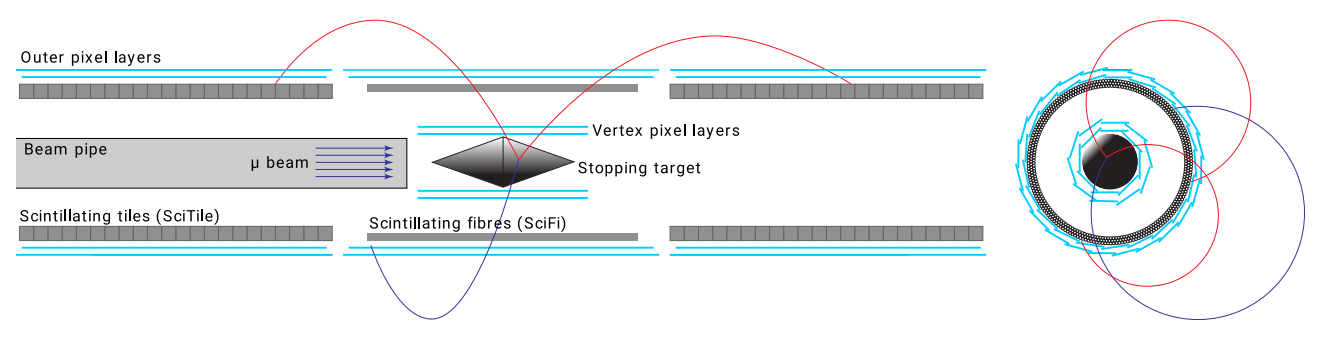
\includegraphics[width=\textwidth]{fig/setup/det.PNG}
    \caption{Figure the layout of the detectors of the Mu3e experiment in the $r-z$ plane, with an example of a $\mu^{+}\xrightarrow{}e^{+}e^{+}e^{-}$ decay \cite{rudzki2021mu3e}.}
    \label{fig:det}
\end{figure}

\subsection*{Beam and Stopping Target}
Phase 1 of the experiment will use the Compact Muon Beam Line (CMBL) based at PSI as this is the only muon beam capable of generating the high rate of muons required to reach the desired sensitivity of the experiment. PSI has a $1.4$MW proton beam which delivers protons of $590$MeV at a current of $2.4$mA \cite{kiselev2021meson} to target E, in the case of Mu3e. Through interactions with the protons in the nuclei of the target material, pions are produced in abundance\cite{berg2016target}. The type of pion produced with the largest abundance is the positive pion and therefore these are selected, and the rest of the decay products are filtered. Of these positive pions, those that have been stopped on the target are selected as they decay to surface muons with enough energy to escape the surface of the target. The reason for selecting these surface muons as opposed to the muons that are generated around the target as well is that they are almost always the same charge \cite{berg2016target}, have a small momentum range and are $\simeq 100\%$ polarized\cite{kiselev2021meson}. Specifically the low momentum of these surface muons allows for accurate control of their momentum and therefore ideal for stopping on thin targets, as is the case in Mu3e. The beam generates close to $10^{8}\mu^{+}/s$ \cite{Calibbi}. This beam is shared between Mu3e and the MEG II experiment. 

\paragraph{}
 The muons from the CMBL are directed to the stopping target situated at the centre of the central station of the Mu3e experiment as shown in figure \ref{fig:det}. The target is a double cone shape as shown in figure \ref{fig:stop}. The purpose of the target is to stop muons in the center of the tracker. By doing this, the initial vertex can be reconstructed from one stationary point and the sum of the momenta of the reconstructed tracks should be equal to zero. The sum of the magnitudes of the momentum of the tracks should also equal the invariant mass of the muon. The final design of the stopping target is given in figure \ref{fig:stop}. Two factors were the focus of the design of the stopping target: maximising stopping power and spreading the decay vertices out as much as possible. In order to maximise stopping power, the amount material in the z-direction needs to be increased as much as possible. This however had to be balanced with the need to minimise material in the way of the tracks to reduce multiple scattering. The other factor was to spread the vertices out as much as possible, this allows for a low occupancy in local areas of the pixel detector and to reduce combinatorial background by decreasing the number of coincidental vertices \cite{Arndt}. The combination of these factors led to the hollow, double cone shape as seen. This design best satisfies these requirements as the angle of the cone allows for the vertices to be spread out along the surface which distributes the decay tracks evenly across the detector. The use of $70-80\mu m$ Mylar allows for minimal photon conversion and multiple scattering which is the largest background source for Mu3e.

\begin{figure}
    \centering
    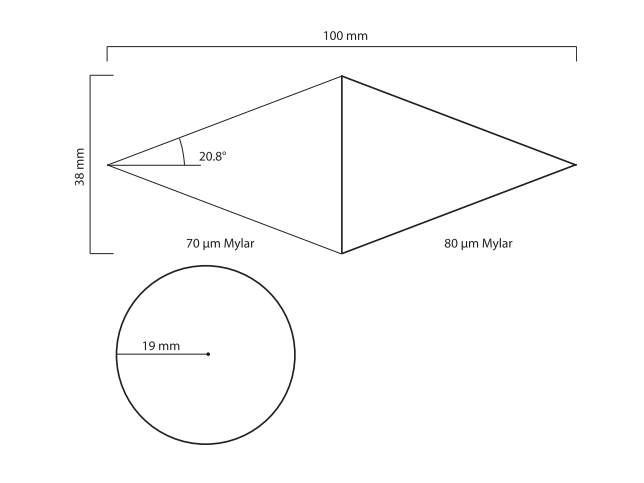
\includegraphics[width=\textwidth]{fig/setup/stop.PNG}
    \caption{Figure showing the dimensions of the stopping target. The upper image is from the $r-z$ plane, the lower from the $x-y$ plane. For the upper image the beam would be incident on the left side of the target \cite{Calibbi}.}
    \label{fig:stop}
\end{figure}

\subsection*{Magnet}
The purpose of the magnet is for particle identification and precise momentum measurements. By having the detector sat inside a magnetic field, the charged decay products are forced into helices that are dependant on their respective charge and momentum. Positrons are propagated in the negative z-direction and electrons in the positive. This field also forces the decay products into helices which allows for longer tracks to be generated. This in turn allows for precise measurements of the momentum as more spatial and temporal information can be collected. The field drives the tracks through the central station and then back into one of the two recurl stations that sit up and downstream of the central detector. In order to achieve the precision required by Mu3e, the chosen magnet is a superconducting $1T$ solenoidal magnet. This must also have an inhomegeniety of $\leq 10^{-3}$ and a stability over 100 days of $\leq 10^{-4}$ \cite{Arndt}.

\subsection*{Scintillating Fibres and Tiles}
Scintillating fibres and tiles are used to provide timing information of the tracks. The suppression of combinatorial background is essential for Mu3e, this is achieved with excellent vertex resolution which in turn is dependant on the timing resolution. As Mu3e uses tracks that recurl back into the detector to gain precise measurements of the momentum, the timing detectors are therefore used to reduce ambiguity in the direction of the tracks as there will be a time difference between tracks exiting and entering the detector. The charge of the decay products can also be identified by the timing detectors. This can be achieved with time of flight measurements and the direction these measurements are taken. Hits in the fibres can be causally related to hits in the tiles and vice versa to identify a common track. Using the spacial information from the timing detectors in combination with the knowledge of the direction of the magnetic field will give charge identification. The timing resolution of the pixel sensors is $\leq 20 ns$ which when combined with the readout time creates event frames that are $64 ns$ (CHECK) long. In order to identify charge a timing resolution of $\leq 500 ps$ is required. In order to temporally separate muon decays in the same frame a resolution of $\leq 100 ps$ is required \cite{Arndt}.

\subsubsection*{Scintillating Fibres}
The scintillating fibres in the central detector are arranged into a series of ribbons that are placed in between the second and third silicon tracking layers. They provide a timing resolution of $250 ps$ with a signal efficiency of $96 \%$ and spatial resolution of $\sim 100 \mu m$ \cite{bravar2022development}. To minimise the effects of multiple scattering and energy loss, the fibres are arranged into ribbons comprised of three layers of $250 \mu m$ thick fibres. This lowers the percentage of the radiation length to $< 0.2\% X\backslash X_{0}$. The primary purpose of the scintillating fibres is separate individual events in frames recorded by the silicon tracker. The secondary is to use time of flight information, as tracks either recurl into the central station or into the recurl stations, to identify the charge of the particle being measured.

\subsubsection*{Scintillating Tiles}
Located in the recurl stations are the tile detectors. 
The tile detectors are arranged in a hollow cylinder, just like the scintillating ribbons. 
As tiles are placed in the recurl stations, they provide timing on the end of tracks and therefore scattering effects and energy loss is not a concern. 
This means a much more efficient material can be used. The material is a $6.3 \times 6.2 \times 5.0 mm^{3}$ plastic scintillator. 
Due to the higher photon yield, the detector efficiency is much higher than the fibres. After calibration, the efficiency was found to be above $99\%$. 
The requirement of the tiles is to have a timing resolution of $\leq 100ps$ \cite{Arndt}, but after testing it was shown the single channel timing resolution was $\approx 47 ps$ \cite{klingenmeyer2020measurements}.

\subsection*{Silicon Trackers}
The silicon tracking layers are used to provide spatial information on the tracks left by the decay products. 
Like the timing detectors, these pixel layers are hollow cylinders arranged concentrically around the beam line. 
These layers in turn are made up of a series of pixel sensors fixed to ladders that lie parallel to one another. 
The sensors themselves are high voltage monolithic active pixel sensors (HV-MAPS) that utilise CMOS technology. 
By using CMOS technology amplification of the signal is done for each pixel individually as seen in figure \ref{fig:pix}. 
Unlike MAPS, HV-MAPS collect charge (deposited by a particle passing through the depletion region) using drift rather than diffusion which allows for much higher time resolution, a critical factor for the Mu3e experiment \cite{schoning2020mupix}. 
The voltage is determined by the resistivity, which in turn is largely determined by the depth of the depletion region. 
This can be thinned to $15-50 \mu m$ which means the total depth of the sensor can be extremely small. 
The thinner the sensor, the amount of material in the decay products path is reduced and therefore the effect of multiple scattering is reduced. 
For phase one of Mu3e, the sensors will be thinned to $50 \mu m$. A final key feature of the sensors for Mu3e is their use of two comparators in parallel in the periphery electronics of the pixel as seen in figure \ref{fig:pix}. 
By doing this two separate signal thresholds can be set, a lower threshold for time information/sampling and a higher threshold for hit validation \cite{augustin2021mupix10}. 
By having these two pieces of information, it allows for low noise (by validating the signal) and low jitter (by using the time information) \cite{schoning2020mupix}. 
The final prototypes of the MuPix sensors showed a hit efficiency of $>99\%$ efficiency \cite{rudzki2021mu3e}.

\begin{figure}
    \centering
    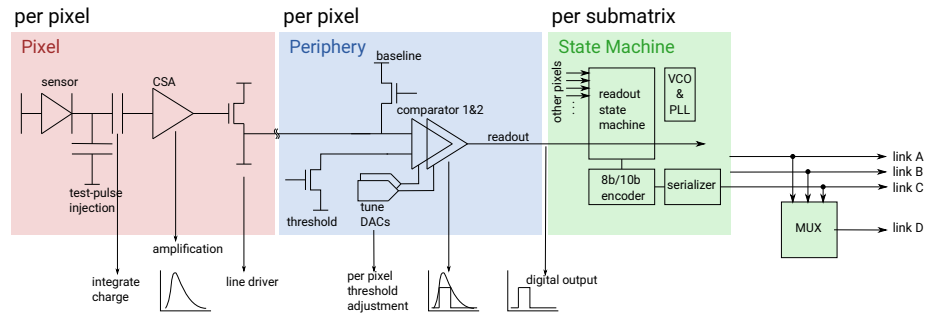
\includegraphics[width=\textwidth]{fig/setup/pix.PNG}
    \caption{Figure showing the pixel architecture for MuPix10 \cite{augustin2021mupix10}.}
    \label{fig:pix}
\end{figure}

\paragraph{}
The arrangement of the pixel tracking layers are shown in figure \ref{fig:det}. 
The two innermost layers are the vertex locator, following from there are the outer layers: two layers in the central detector, and two layers in each recurl station. 
The purpose of the layers is to collect hits from the decay products and provide spacial and temporal information on these hits.

\section*{Tracking in the Mu3e Experiment}
The Mu3e experiment sits in a homogenous solenoidal magnetic field centered around the z-axis. In this setup, a right-handed coordinate system is used with the z-axis sat parallel to the direction of the magnetic field. 
This setup forces the decay products into a characteristic helix, from which the momenta and thus the energy of these particles can be derived.
As stated, calculation of the momenta of the tracks, in conjunction with the geometrical properties of the decay vertex, are used to identify potential signal events.
The physical background events are internal conversion. In order to discriminate these background events from signal an excellent momentum resolution is required (1 Mev \cite{MartinPerez2023}).
\subsection*{Geometrical Foundation of Tracking}
The charged products of the signal decay are forced into helices by the magnetic field centered on the z-axis of the experiment.
By parameritising the geometrical properties of a given helix, spatial information of hits in the detector can be used to draw the shape of the tracks of these products and thus energy and momenta can be calculated.
The first task is to factorise out the circular fit of the tracks in the x-y plane and the linar fit in the z axis.
From the basic fit of a helix, the uncertainty due to multiple scattering is incorporated.
The parameterisation of the helices follows the method given by \cite{KARIMAKI1991187} and visualised in figure \ref{fig:bend}. 
As seen in figure \ref{fig:bend} three points are taken in successive silicon tracking layers, through which an arc can be drawn.
From this arc, an uncertainty must be introduced due to multiple scattering as the particle passes through the tracking layers.
By assuming momentum is conserved, the radius of curvature is constant and all that must be calculated is the spatial difference between the two centres of the arc.
By calculating this difference, a corrective angle due to multiple scattering can be derived, as denoted in figure \ref{fig:bend} by $\Phi_{MS}$.
By applying a straight line fit in the $s-z$ plane to construct a total helix, a corresponding corrective angle can be applied for the perpendicular plane, given by $\Theta_{MS}$.
In the Mu3e experiment, only the uncertainty due to multiple scattering is taken into account. This therefore leads to the challenge of finding a three-dimensional curvature that minimises equation \ref{eq:chi2}
\begin{equation}
    \chi^{2}(R_{3D}) = \frac{\Phi_{MS}(R_{3D})^2}{\sigma_\phi^2} + \frac{\Theta_{MS}(R_{3D})^2}{\sigma_\theta^2}
    \label{eq:chi2}
\end{equation}
The radius of this arc is denoted with $r$ and the opening angle between the first and last hit is given by $\Phi$.
By introducing bending angles and corrective parameters from multiple scattering each pair of hits has an associated radius and and centre.
To construct larger tracks, a series of triplets that share hits in the silicon trackers are combined. The $\chi^2$ function of the longer tracks is the summation of the $\chi^2$ equation \ref{eq:chi2} for each of the constitiuent triplete due to each scatter being independant of each other.
In practice, the procedure is to collect all the relevant hits for a given track, fit each triplet individually and then calculate the summation of these $\chi^2$ values. Throughout the process of finding relevant hits, selection cuts are applied to the track.
These selection cuts are initially focused on the spatial position of the successive hits, from this a cut is applied on the tangential radius. After the fitting has been completed for the track a cut is made on the $\chi^2$ value.
Every track that passes this set of criteria is passed to the vertex fitter.
\begin{figure}
    \centering
    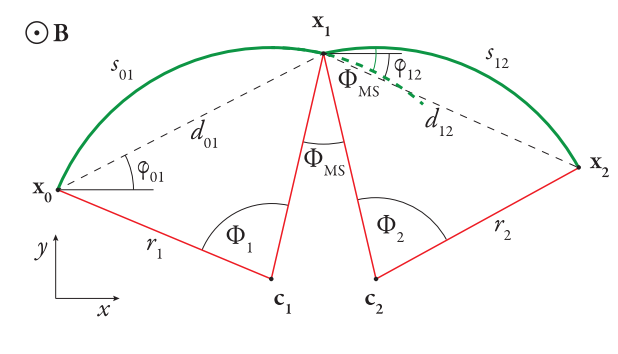
\includegraphics[width=10cm]{fig/tracking/bending.PNG}
    \caption{Figure visualising the tracking parameters associated with the circular fit in the x-y plane. Where $r$ denotes the radius of the arc, $c$ denotes the centre of the arc and $\Phi$ is the opening angle of the arc. \cite{berger2017new}.}
    \label{fig:bend}
\end{figure}
	%---------------------------------------------------
	%\part{Analyses}
	%Analyses
        \part{Silicon Hit Efficiency Study}
        \section{Motivation}
\textbf{
    \begin{itemize}
        \item Discuss the meaning behind silicon hit efficiency.
        \item Why does it need to be measured (high intensity experriment etc)
        \item Why is it done through tracking.
        \item How can this statistic be used?
    \end{itemize}
}
The Mu3e experiment is 

\section{Silicon Hit Inefficiency}
\textbf{
    \begin{itemize}
        \item Reiterate what is meant by silicon hit efficiency.
        \item How is this implemented in the software.
        \item Discuss how this issue might present itself in the experiment.
    \end{itemize}
}
The silicon hit efficiency refers to the proportion of hits that are incident on a sensor and are recorded, for instance a $75\%$ efficient detector would record $75\%$ of the hits that are incident on it. In the software, this inefficiency is introduced when mapping the hits at the track reconstruction level. After the simulation has finished, the hits are collected along with spatial and temporal coordinates. As this mapping process is underway, an inefficient layer is selected, as is a silicon hit efficiency. When the hits in the inefficient layer are being mapped, a random number is used to decide whether the hit is mapped. Under the current algorithm, the inefficiency is introduced as a uniformly distributed frequentist function. 
\begin{equation}
    \text{Hit Efficiency} = \frac{\text{Recorded Hits}}{\text{Number of Hits in Layer}}
\end{equation}
This was chosen for the purpose of understanding the effect that each layer had on the reconstruction.
\section{Ordering of the Algorithm}
\textbf{
    \begin{itemize}
        \item This needs to be cleaned up, with a better title.
        \item Show that the black boxes are what happens in the nominal algorithm.
        \item Reiterate how an inefficieny is simulated and how the backwards propagation works.
    \end{itemize}
}
The ordering of this algorithm is shown below. In order to measure the efficiency of the silicon tracking layers without using truth information and run over real data. As shown in the diagram below, the reconstruction algorithm follows the same process as the nominal reconstruction algorithm. The process uses a series of nested loops to move from each layer and attempt to fit a track to an increasing number of hits. In the diagram, the black boxes represent the common processes between the two algorithms, the red boxes represent the changes that are introduced.
\par
When running over real data, the 'test layer' is skipped and a five-hit track is reconstructed. After the track is reconstructed, the geometric features of the track are used to propagate back to the test layer. Within a specified z and $\phi$ range around the track on the test layer, a hit is either found or not found. It is using this ratio whereby a hit efficiency is calculated.
\usetikzlibrary{arrows,positioning,shapes.geometric}
    \begin{tikzpicture}[>=latex']
        \tikzset{block/.style= {draw, rectangle, align=center,minimum width=2cm,minimum height=1cm},
        rblock/.style={draw, shape=rectangle,rounded corners=1.5em,align=center,minimum width=2cm,minimum height=1cm},
        input/.style={ % requires library shapes.geometric
        draw,
        trapezium,
        trapezium left angle=60,
        trapezium right angle=120,
        minimum width=2cm,
        align=center,
        minimum height=1cm
    },
        }
        \node [rblock]  (start) {Geant4 Simulation};
        \node [rblock, right =1cm of start] (acquire) {Sort Hits into Frames};
        \node [block, right =1cm of acquire] (rgb2gray) {Map Hit Information: \\ Positional and Temporal};
        \node [block, above =1cm of rgb2gray, draw=red] (mod) {Remove Hits: \\ Positional and Temporal Information};
        \node [block, below =1.5cm of start] (otsu) { Make Doublets: \\ Pairs of Hits in Consecutive Layers};
        \node [rblock, right =1cm of otsu] (gchannel) {Begin Reconstruction:\\Start from the Inner Layer};
        \node [block, below =1.5cm of otsu] (closing) {Make 4 Hit Segments: \\ 2 Triplets};
        \node [block, right =1cm of closing] (hit) {Make 6 Hit Segments: \\ 4 Triplets};
        \node [block, right =1cm of hit] (hits) {Make 8 Hit Segments: \\ 4 Triplets};
        \node [block, left =1cm of mod, draw=red] (mod5) {Artifical Inefficiency: \\Silicon Hit Efficiency, Test Layer and Test Station};
        \node [input, below left=1.5cm and 0.01cm of hit] (limit) {Merge Tracks that have Shared Hits};
        \node [block, below right =0.15 and 2cm of gchannel,draw=red] (mod2) {Skip Test\\ Layer};
        \node [coordinate, below right =0.75cm and 0.6cm of rgb2gray] (right) {};  %% Coordinate on right and middle
        \node [coordinate,above left =0.75cm and 0.6cm of otsu] (left) {};  %% Coordinate on left and middle
        \node [coordinate, below right =0.75cm and 0.6cm of gchannel] (right2) {};  %% Coordinate on right and middle
        \node [coordinate,above left =0.75cm and 0.6cm of closing] (left2) {};  %% Coordinate on left and middle
        \node [coordinate, below right =0.75cm and 0.6cm of hits] (right3) {};  %% Coordinate on right and middle
        \node [coordinate,above left =0.75cm and 5.5cm of limit] (left3) {};  %% Coordinate on left and middle
        \node [coordinate, left =1.5cm of right3] (right4) {};  %% Coordinate on left and middle
        \node [block, below =0.75cm of right4,draw=red] (mod3) {Propagate Backwards: \\Find Missing Hit};
        \node [block, below =0.75cm of mod3,draw=red] (mod4) {Assign Z and $\phi$ limits \\To Search in};

%% paths
        \path[draw,->] (start) edge (acquire)
                    (acquire) edge (rgb2gray)
                    (rgb2gray.east) -| (right) -- (left) |- (otsu)
                    (otsu) edge (gchannel)
                    (gchannel.east) -| (right2) -- (left2) |- (closing)
                    (closing) edge (hit)
                    (hit) edge (hits)
                    (hits.east) -| (right3) -- (left3) |- (limit)
                    
                    ;
        \path[draw=red,-] (mod4) edge (mod3)
                        (mod) edge (rgb2gray)
                        (mod2) edge (right2)
                        (mod3) edge (right4)
                        (mod5) edge (mod)
                    ;
    \end{tikzpicture}

\section{Matching Algorithm}
\textbf{
    \begin{itemize}
        \item Needs to discuss what is defined as a 'matched' track and what a 'truth' track.
        \item Why is it important to measure and have a high matching efficiency? (Picking important parameter range)
        \item What does a high matching efficiency mean for the experiment?
    \end{itemize}
}
When the track is propagated back to the test layer and a hit is either found or not, this ratio of hits found or not found is used to calculate the hit efficiency. In order to trust that this ratio is correct, the track must either match to the nominal algorithm or be a truth track. An algorithm is written such that the tracks are reconstructed together and a matched based on common hits. A track is considered as matched if it either matches to a track reconstructed by the nominal algorithm or it is truth. If it matches to the nominal algorithm, it can be assumed that if a hit is found or not found this can be used to assess the silicon hit efficiency of the layer. If it doesn't match to the nominal tracking but it is a truth track, this can be assumed that it is passing through an intrinsic inefficiency in the layer.
\par
Using this matching algorithm, a matching efficiency can be calculated and plotted against multiple variables associated with the tracks. This is done to find regions in parameter space whereby the matching efficiency is extremely high. By doing this, cuts can be applied when completing the reconstruction over real data and it can be assumed that all the tracks are correct.
\begin{figure}
    \centering
    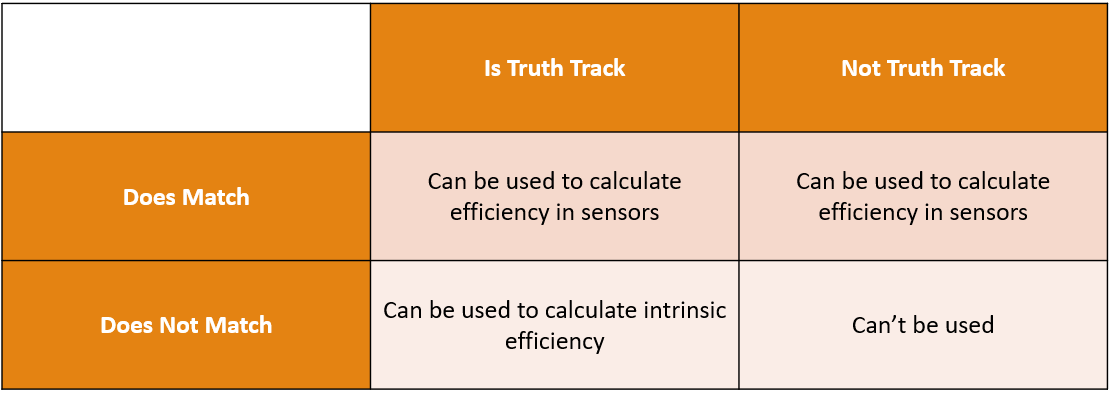
\includegraphics[scale=0.6]{fig/match/Capture.PNG}
    \caption{Table showing the type of track produced by the modified reconstruction algorithm and what it can be used for.}
    \label{fig:table}
\end{figure}
\begin{figure}
    \centering
    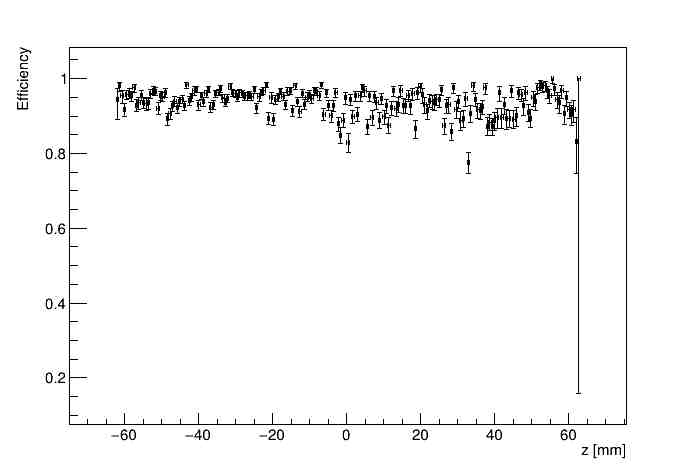
\includegraphics[scale=0.6]{fig/match/prop_z_eff.jpeg}
    \caption{Matching efficiency as a function of prop z.}
    \label{fig:mpz}
\end{figure}
\begin{figure}
    \centering
    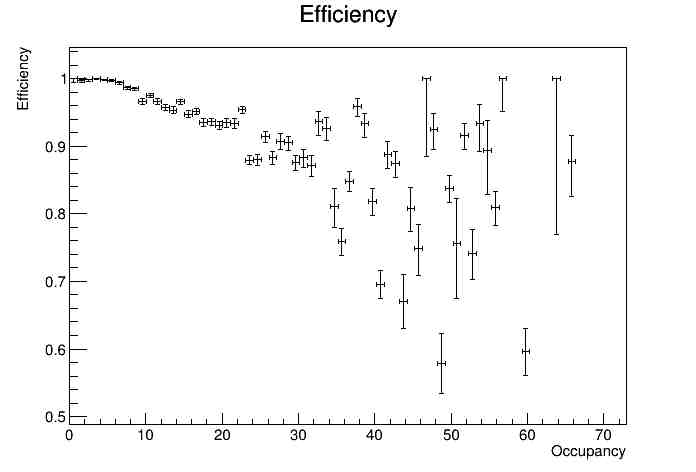
\includegraphics[scale=0.6]{fig/match/effic_nhit.jpeg}
    \caption{Matching efficiency as a function of occupancy.}
    \label{fig:occ}
\end{figure}
\begin{figure}
    \centering
    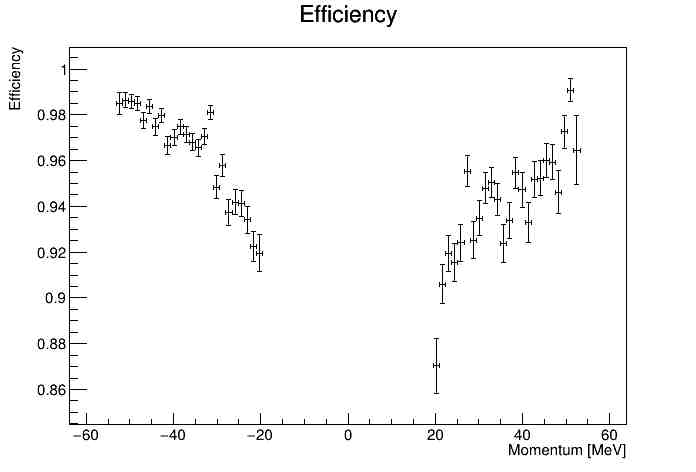
\includegraphics[scale=0.6]{fig/match/effic_p.jpeg}
    \caption{Matching efficiency as a function of momentum.}
    \label{fig:effp}
\end{figure}
\section{Z and $\phi$ Range}
After reconstruction, the parameters of the track are used to propagate the track to a position on the test layer. A preset z and $\phi$ range are then used to locate a hit close to the position of the track. With the assumption that the tracks are either matched to a nominal track or a truth track, if a hit is found or not found, it is because the hit is either there or not there.  Also mention the relationship between the window and the resolution. What is the associated error that will be accumulated if the resolution is improved. 
\begin{figure}
    \centering
    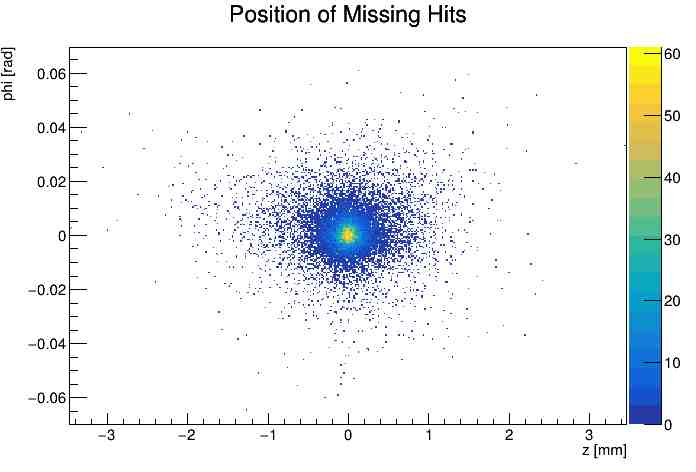
\includegraphics[scale=0.6]{fig/match/position.jpeg}
    \caption{Matching efficiency as a function of momentum.}
    \label{fig:pos}
\end{figure}
\begin{figure}
    \centering
    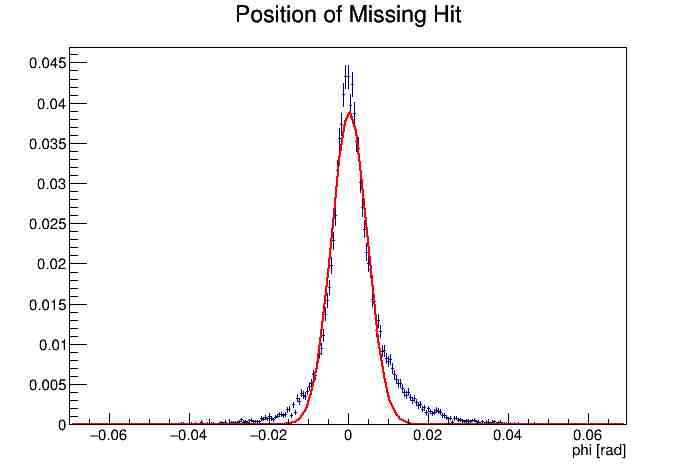
\includegraphics[scale=0.6]{fig/match/position_phi.jpeg}
    \caption{Matching efficiency as a function of momentum.}
    \label{fig:effp}
\end{figure}
\section{Efficiency Heat Maps}
\textbf{
    \begin{itemize}
        \item Go through how the efficiency is calculated.
        \item Move to interesting features (intrinsic inefficiencies and overlap).
        \item Discuss the fiducial region.
    \end{itemize}
}

\begin{figure}
    \centering
    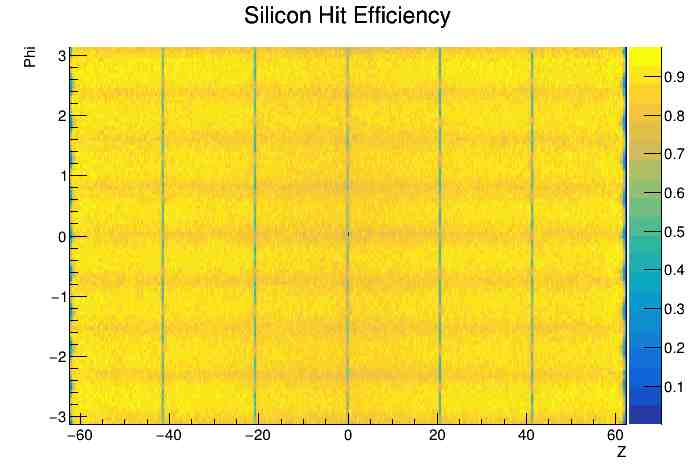
\includegraphics[scale=0.6]{fig/eff/final_eff.jpeg}
    \caption{90\% hit efficiency heat maps.}
    \label{fig:effp}
\end{figure}
\begin{figure}
    \centering
    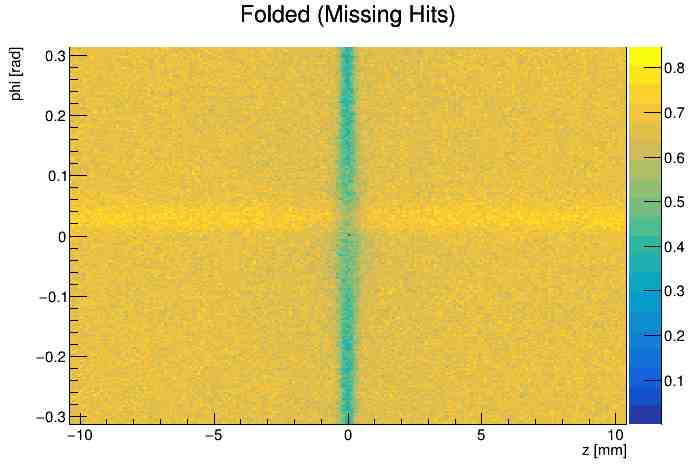
\includegraphics[scale=0.6]{fig/eff/folded_75.jpeg}
    \caption{Folded plot of 75\% hit efficiency.}
    \label{fig:effp}
\end{figure}
\section{Calculation of Hit Efficiency}
\textbf{
    \begin{itemize}
        \item This needs to be completely redone.
        \item The error derivation needs to be done here, Bayesian derivation and error estimation.
    \end{itemize}
}
Go through Bayesian derivation of the errors. Matching efficiency and z and $\phi$ windows
\begin{equation}
    Pr(A|B) = \frac{Pr(B|A)Pr(B)}{Pr(B)}
\end{equation}
\begin{equation}
    Pr(H|M) = \frac{Pr(M|H)Pr(H)}{Pr(M)}
\end{equation}
\section{Effect of Efficiency on Chi Squared Distribution}
\textbf{
    \begin{itemize}
        \item This should be the final stop, the actual presentable effect of an inefficiency.
    \end{itemize}
}
\begin{figure}
    \centering
    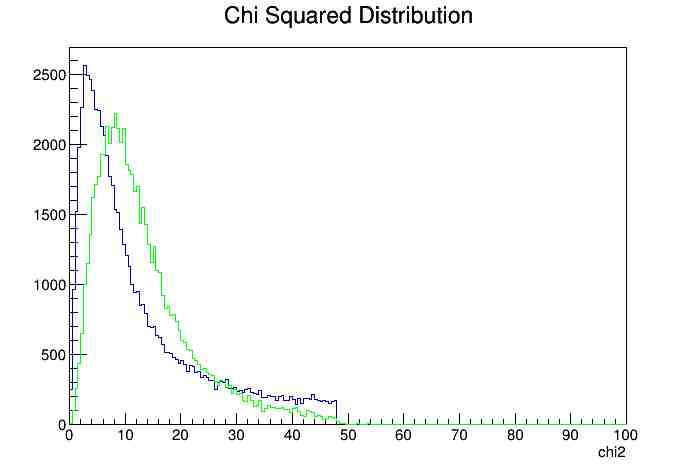
\includegraphics[scale=0.6]{fig/eff/chi2.jpeg}
    \caption{Effect of 70\% efficiency.}
    \label{fig:chi2}
\end{figure}
        \part{Alternative Tracking Algorithm}
        \section{Motivation}
\textbf{
    \begin{itemize}
        \item This should be discussed as an extension to the previous study.
        \item The plots should show the proportional relationship between hit efficiency and reconstruction efficiency.
        \item Discuss why it is important to recover tracks (high intensity experiment etc)
    \end{itemize}
}
In the Mu3e experiment the number of tracks recorded is directly proportional to the ratio between the number of hits that should be recorded in the silicon detector and the number of hits actually recorded. 
Figure \ref{fig:hit_eff} shows the relationship between the reconstruction efficiency and the hit efficiency. Whereby the hit efficiency is defined as the ratio between the number of hits recorded in the detector and the number of Monte Carlo (MC) truth hits. The reconstruction efficiency is defined as the number of tracks recorded normalised by the number of tracks recorded at $100\%$ hit efficiency.
\begin{figure}
    \centering
    \begin{subfigure}{.5\textwidth}
        \centering
        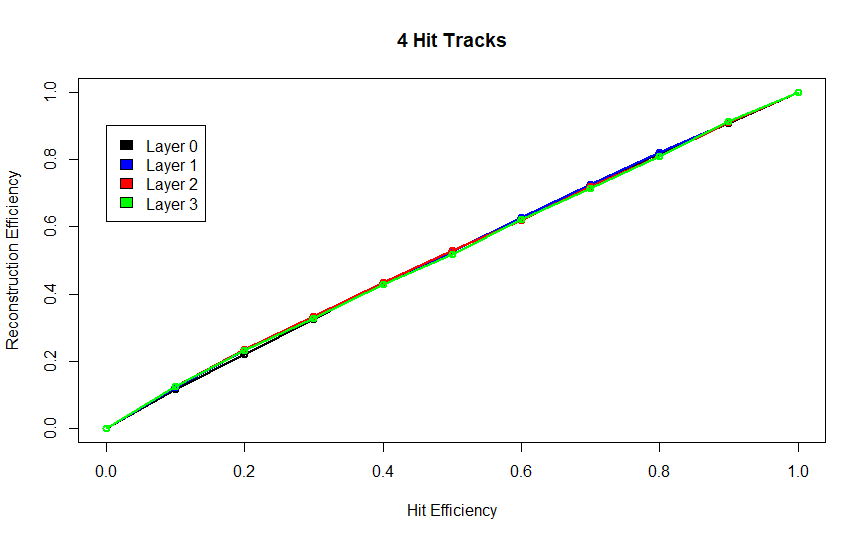
\includegraphics[scale=0.3]{fig/eff/4.png}
        \caption{Plots showing the relation between reconstruction efficiency and the hit efficiency.}
        \label{fig:eff4}
    \end{subfigure}%
    \begin{subfigure}{.5\textwidth}
        \centering
        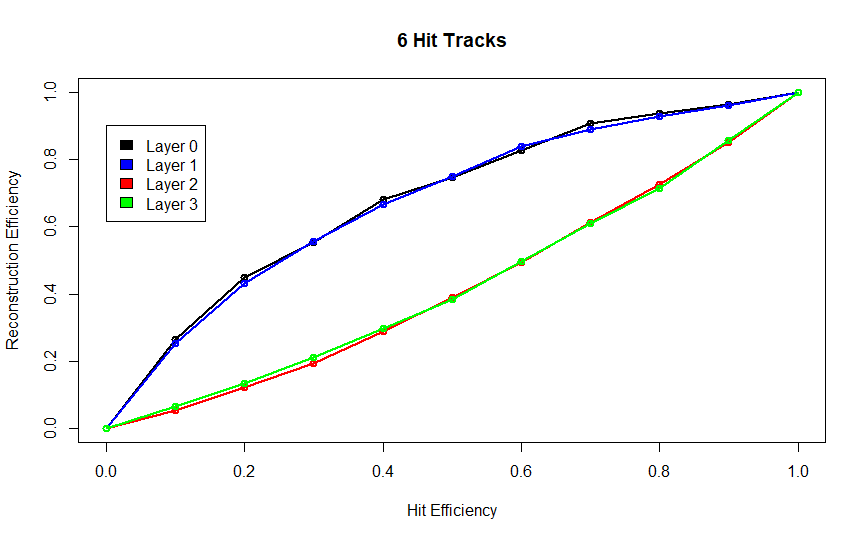
\includegraphics[scale=0.3]{fig/eff/6.png}
        \caption{Plots showing the relation between reconstruction efficiency and the hit efficiency.}
        \label{fig:eff6}
    \end{subfigure}
    \caption{The above figures show the effect a given hit efficiency has on the reconstruction efficiency for tracks that are both 4 and 6 hits long. Hit efficiency is defined as the ratio between the number of hits recorded in the detector and the total number of Monte Carlo hits. Reconstruction is defined as the total number of tracks generated at a given hit efficiency divided by the number of tracks generated with 100\% hit efficiency.}
    \label{fig:hit_eff}
\end{figure}
\section{Ordering of the Algorithm}
\textbf{
    \begin{itemize}
        \item You should use the top flowchart but redesign it in latex
        \item The number of subsections after this should be reduced.
    \end{itemize}
}
In this section, the order of the algorithm is discussed. 
Seen below is a flowchart where the order of the algorithm is summarised.
\par
\begin{figure}
    \centering
    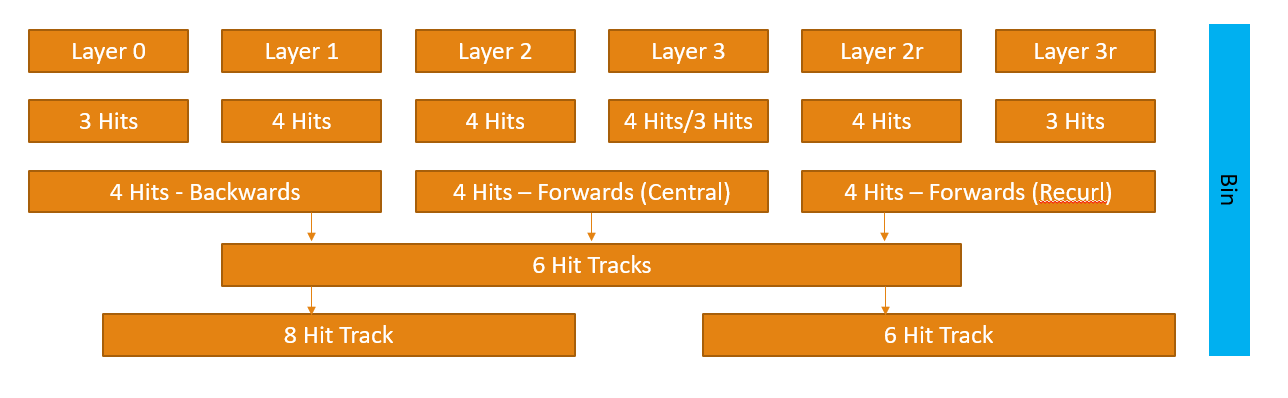
\includegraphics[scale=0.6]{fig/tracking/flow.png}
    \caption{This might be a better flowchart.}
    \label{fig:alt_flow}
\end{figure}
\usetikzlibrary{arrows,positioning,shapes.geometric}
    \begin{tikzpicture}[>=latex']
        \tikzset{block/.style= {draw, rectangle, align=center,minimum width=2cm,minimum height=1cm},
        rblock/.style={draw, shape=rectangle,rounded corners=1.5em,align=center,minimum width=2cm,minimum height=1cm},
        input/.style={ % requires library shapes.geometric
        draw,
        trapezium,
        trapezium left angle=60,
        trapezium right angle=120,
        minimum width=2cm,
        minimum height=1cm
    },
        }
        \node [block]  (start) {Run the Simulation and \\ Collect Hits in Layers};
        \node [block, right =1cm of start] (acquire) {Sort Hits into Frames};
        \node [block, right =1cm of acquire] (rgb2gray) {Map Hit Information: \\ Positional and Temporal};
        \node [block, below =1.5cm of start] (otsu) {Make Initial Triplets \\ for Each Layer: Link $\xrightarrow{}$ \ref{tab:1}};
        \node [block, right =1cm of otsu] (gchannel) {Divide each list of triplets into \\ smaller momentum ranges: Link $\xrightarrow{}$ \ref{2}};
        \node [rblock, right =1cm of gchannel] (closing) {Connect triplets together \\ from the Layer 2 triplets:  \\ Link $\xrightarrow{}$ \ref{3}};
        \node [block, below =1.5cm of otsu] (hit) {Make 4 hit tracks from triplets \\ before and after layer 2: Link $\xrightarrow{}$ \ref{4}};
        \node [block, right =1cm of hit] (hits) {Connect tracks together for \\ 6 hit tracks: Link $\xrightarrow{}$ \ref{5}};
        \node [block, below=1.5cm of hits] (limit) {Connect 6 hit tracks for 8 \\ hit tracks: Link $\xrightarrow{}$ \ref{6}};
        \node [coordinate, below right =0.75cm and 0.6cm of rgb2gray] (right) {};  %% Coordinate on right and middle
        \node [coordinate,above left =0.75cm and 0.6cm of otsu] (left) {};  %% Coordinate on left and middle  %% Coordinate on right 
  %% Coordinate on left and middle
        \node [coordinate, below right =0.75cm and 0.6cm of hits] (right3) {};  %% Coordinate on right and middle
        \node [coordinate,above left =0.75cm and 5.5cm of limit] (left3) {};  %% Coordinate on left and middle
        \node[coordinate, below = 0.75cm of closing] (right2){};
        \node[coordinate, above left = 0.75cm and 0.6cm of hit] (left2){};


%% paths
        \path[draw,->] (start) edge (acquire)
                    (acquire) edge (rgb2gray)
                    (rgb2gray.east) -| (right) -- (left) |- (otsu)
                    (otsu) edge (gchannel)
                    (gchannel) edge (closing)
                    (closing.south) -| (right2) -- (left2) |- (hit)
                    (hit) edge (hits)
                    (hits.east) -| (right3) -- (left3) |- (limit)
                    
                    ;
                    ;
    \end{tikzpicture}

\subsection{Initial Triplets}
Initially triplets are formed from each layer. Seen below is the start layer of each triplet and the layers that triplet passes through. In the table, lower case r refers to a recurl station layer.
\vspace{0.3cm}
\begin{center}
\begin{tabular}{||c c c c c c||} 
 \hline
 Layer 0 & Layer 1 & Layer 2 & Layer 3 & Layer 3r & Layer 2r \\ [0.5ex] 
 \hline\hline
 0,1,2 & 1,2,3 & 2,1,0 & 3,2,1 & 3r,3,2 & 2r,3r,3 \\ 
 \hline
  &  & 2,3,3 & 3,3,2 &  &  \\
 \hline
  &  & 2,3,3r & 3,3r,2r &  &   \\
 \hline
\end{tabular}
\label{tab:1}
\end{center}
\subsection{Dividing Triplets into Smaller Ranges}
\label{2}
The purpose of this is to reduce the number of tracks that have to be sorted through and hopefully just leave triplets that correspond to the same track in each frame. In order to quickly divide up these tracks a parameter was needed that was global because local parameters would mean that triplets starting from each layer would not correlate to each other. For this reason, the 3-dimensional curvature parameter was chosen. It is this parameter that is then used to calculate the radii of the tracks and therefore the momentum. The current issue is that the error on this parameter is quite large relative to the range of curvature values meaning there is a chance that some triplets are not being matched because of the size of the ranges.
\subsection{Connect Triplets to the Layer 2 Triplets}
\label{3}
From the initial triplets we want to make longer tracks. Initially we start by looking at the triplets from layer 2 as this is a good center point. Triplets from this layer will have overlapping hits from triplets from each layer. Layer 2 has triplets pointing both forward and backwards. In the following tables the both the forward and backward layers are shown with the triplets that are connected with the final track that is left and the order of hits.
\vspace{0.3cm}
\begin{center}
\begin{tabular}{||c c c c c||}
 \hline
 & & $\boldsymbol{Backward}$ $\boldsymbol{Triplets}$& & \\
 \hline\hline
 Layer 2 Triplet & Other Layer & Other Layer Triplet & Length & Hit Order \\ [0.5ex] 
 \hline\hline
 2,1,0 & 1 & 1,2,3 & 4 & 0,1,2,3 \\ 
 \hline
 2,1,0 & 0 & 0,1,2 & 3 & 0,1,2 or 2,1,0 \\
 \hline
 2,1,0 & 3 & 3,2,1 & 3 & 0,1,2,3 \\
 \hline
\end{tabular}
\end{center}
\vspace{0.5cm}
\begin{center}
\begin{tabular}{||c c c c c||}
 \hline
 & & $\boldsymbol{Forward}$ $\boldsymbol{Triplets}$& & \\
 \hline\hline
 Layer 2 Triplet & Other Layer & Other Layer Triplet & Length & Hit Order \\ [0.5ex] 
 \hline\hline
 2,3,3 & 3 & 3,3,2 & 3 & 2,3,3 or 3,3,2 \\ 
 \hline
 2,3,3r & 3r & 3r,3,2 & 3 & 2,3,3r or 3r,3,2 \\
 \hline
 2,3,3r & 2r & 2r,3r,3 & 4 & 2,3,3r,2r \\
 \hline
 2,3,3 & 2 & 2,3,3 & 4 & 2,3,3,2 \\
 \hline
\end{tabular}
\end{center}
\subsection{Connect the Triplets into 4 Hit Segments Before and After Layer 2}
\label{4}
Now there are longer tracks from both the forward and backward triplets from layer 2, we combine them to make 4 hit tracks either in the central layer or re-curling back into one of the stations. The tracks and the order of the hits is shown below. Along the way triplets that don't align with these 4 hit segments will be put into a bin list as it could be due to an inefficiency.
\vspace{0.3cm}
\begin{center}
\begin{tabular}{||c c c c c||}
 \hline
 & & $\boldsymbol{Four}$ $\boldsymbol{Hits}$& & \\
 \hline\hline
 Hit Order & Central Station? & Recurl Station? & Recurl? & Name of List \\ [0.5ex] 
 \hline\hline
 0,1,2,3 & Yes & No & No & s4 \\ 
 \hline
 2,3,3,2 & Yes & No & No & l2\_2\\
 \hline
 2,3,3r,2r & Yes & Yes & Yes & l2r\_2\\
 \hline
\end{tabular}
\end{center}
\subsection{Connect the 4 Hit Tracks to 6 Hit Tracks}
\label{5}
From here we combine the 4 hit tracks into 6 hit tracks. We take the tracks from the s4 list and check it against the other two lists (l2\_2 and l2r\_2). There are two overlapping hits in layers 2 and 3. The result of this should be a subset of 6 hit tracks. Again there should be a series of 4 hit segments that are just 4 hit segments, these are put into a bin list and can be used to look for inefficient tracks.
\subsection{Combine 6 Hit Tracks into 8 Hit Tracks}
\label{6}
There are now 6 hit tracks exclusively in the central station (0,1,2,3,3,2). If an 8 hit track can be formed there should be two 6 hit tracks with overlapping hits in layers 2,3,3,2. If these hits perfectly overlap and the track fits an 8 track can be generated.
\section{Identification of Inefficiency}
\textbf{
    \begin{itemize}
        \item What effect would an inefficiency have on the nominal tracking?
        \item How are inefficiencies identified? 
        What shows up in the alternative tracking?
    \end{itemize}
}
\section{Generating 5 Hit Tracks}
\textbf{
    \begin{itemize}
        \item Discuss what a 5 hit track should look like and why 5 hit.
        \item How are they generated? Where do they come from?
        \item The cuts specific to 5 hit tracks should be discussed here.
    \end{itemize}
}
After the 'complete' tracks have been found, there can be a movement to find the partial tracks.
These can be found from unused shorter tracks. The most simple extension that can be made is from a 4-hit track to a hit in a subsequent layer.
The initial way to do this is to take a 'floating' 4-hit track, as seen in figure \ref{fig:s4}. These can be combined with a triplet from a subsequent layer to form a 5 hit track
as seen in figure \ref{fig:4_5}. Using the same list of floating 4-hit tracks, if a triplet cannot be found to connect to the track, it suggests an inefficiency is present in the given layer.
Instead of connecting said triplet, the given layer is skipped and the fifth hit is found in a subsequent layer.
As in the previous study, we use the already derived geometrical properties of the track to look to the next layer. By using these properties, we can derive a trajectory of the track and estimate the position of a track on a given layer.
Seen in figure \ref{fig:pos}, we can see the difference between our estimation of the position of the hit, derived from the trajectory of the track, and the actual position of said hit.
Using this, an estimation of the position of the fifth hit can be made. By searching for a hit in a range dictated by figure \ref{fig:pos} a five hit track can be generated.
These two methods allow for 4 of the 6 layers to be looked over, said layers being the innermost and the two recurl stations.

In order handle inefficiencies in the outermost layers of the central detector, multiple methods are used.
Initially, a four hit track starting at the innermost layer. As was done when using the floating 4 hit tracks, either a connected triplet is used or the track is propagated past the next layer to a subsequent layer. Finally, triplets from the innermost layer can be connected to 2 seperate hits after a test layer to look past an inefficiency.
Using these methods, inefficiencies in a given test layer can be identified and skipped past.

\begin{figure}
    \centering
    \begin{subfigure}{.5\textwidth}
      \centering
      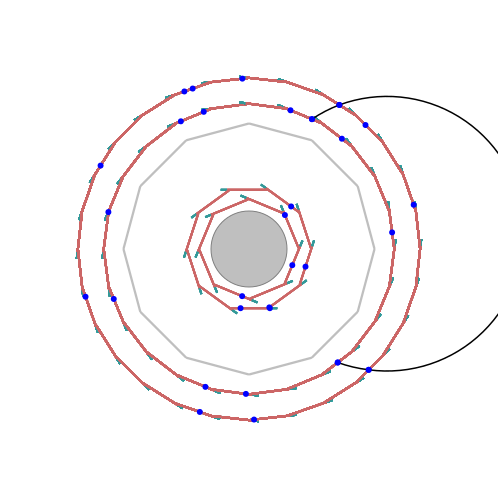
\includegraphics[width=.75\linewidth]{fig/tracking/s4.png}
      \caption{Figure showing an example of a 'floating' 4-hit track.}
      \label{fig:s4}
    \end{subfigure}%
    \begin{subfigure}{.5\textwidth}
      \centering
      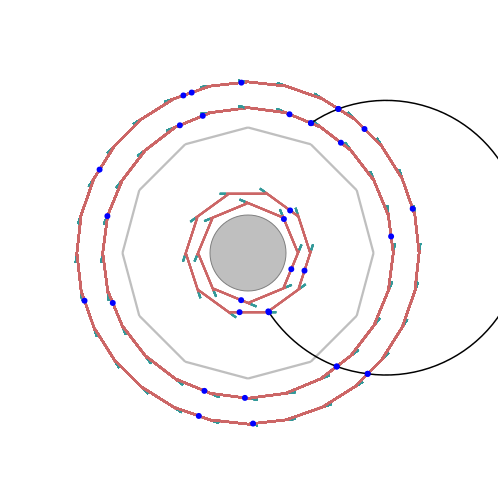
\includegraphics[width=.75\linewidth]{fig/tracking/s5.png}
      \caption{Figure showing the same floating 4-hit track that has been extended to a 5-hit track.}
      \label{fig:s5}
    \end{subfigure}
    \caption{The above figures show the detector in the x-y plane with an example track superimposed over. 
    In this, the above track is extended from a 'floating' 4-hit track to a 5-hit track. This is described as a floating 4-hit track as the track contains no hits in the innermost layer.}
    \label{fig:4_5}
\end{figure}
\subsection{Selection Cuts Applied to the 5 Hit Tracks}
Selection cuts must be applied to the 5 hit tracks in order to improve the purity. As there is a significantly larger distance that the particles are traversing between recorded hits in the detector, the fitting parameters must be less constrained as to allow a greater uncertainty due to multiple scattering.
\subsubsection{$\chi^{2}$ Minimisation}
Due to the lower fitting parameters of the 5 hit tracks, a four hit track that is being extended can be fitted multiple times, either with a triplet from a subsequent layer or a hit from the layer following. If the algorithm is successfully identifying a missing hit then only one of these generated tracks is correct.
By allowing a floating 4 hit track to run through all of the above methods and selecting the track with the lowest $\chi^{2}$ value, the purity is significantly increased.
\subsubsection{Propagation Cut}
For tracks where an individual hit is found, a cut is applied to find hits within a given window on a test layer.
\subsection{Effect on the Purity}
In this bit I want to talk about the number of tracks that have an inefficiency in a given test layer. The plot should show that the number of 5 hit tracks should be inverse to the test layer. Work in progress.
It currently shows there is a massive difference between the first layer and second. It also shows the purity to be rubbish in these sections.
\begin{figure}
    \centering
    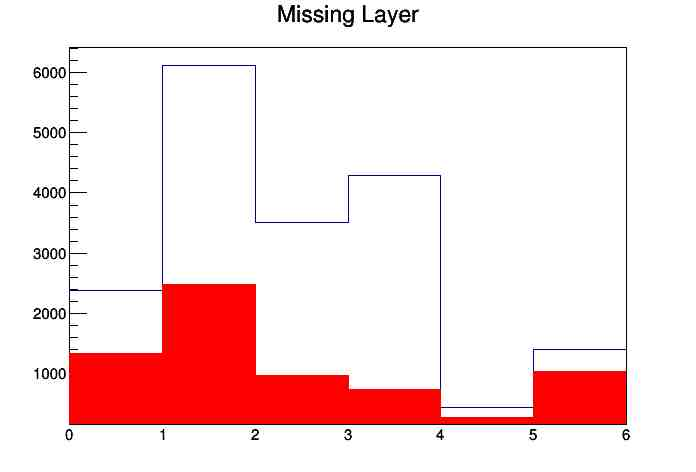
\includegraphics[scale=0.5]{fig/tracking/l.jpeg}
    \caption{Figure showing the number of 5 hit tracks and the inefficient layer that they are attached to. The red bar shows the number of pure tracks and blue shows the total number of tracks.}
    \label{fig:lay}
\end{figure}
\section{Validity of the 5 Hit Tracks}
\textbf{
    \begin{itemize}
        \item This should show the 5 hit tracks can be used.
        \item Discuss the momentum resolution with reference to the minimum resolution of tracks and compare to the 4, 6 and 8 hit track resolutions.
        \item This should also be where the proof that it can be used to vertex should be done.
    \end{itemize}
}
In this section, the use of five hit tracks is to be discussed. The purpose of the tracking is to accurately describe the trajectory of the decay products and calculate the respective momenta and energy.
By reconstructing the trajectory of tracks, vertices can be fitted to given decays and relevant frames can be saved to an offline database for further analysis. 
The secondary purpose of deriving the momenta of these tracks allows for background events to be rejected.
With these two purposes in mind, the assessment of the usefulness of these five hit tracks must be made using these two arguments. 
\subsection{Momentum Resolution}
The momentum of a track is calculated from the transverse curvature of the track and the linear projection along the z-axis.
Associated with the momenta of the tracks is a resolution calculation. This is based of the multiple scattering model provided and the number of layers a given track passes through.
For the purpose of this calculation, Monte Carlo information can be used to make a direct comparison.
\begin{equation}
    \sigma _{p} = \frac{p - p_{mc}}{p}
    \label{eq:res_mome}
\end{equation}
Equation \ref{eq:res_mome} describes the relation between the measured momentum of the track and the resolution of the measured momentum.
Where $\sigma _{p}$ is the resolution of the measured momentum, $p$ is the momentum of the particle in MeV and $p_{mc}$ is the true momentum.
In order to calculate the momentum resolution, equation \ref{eq:res_mome} was plotted as a function of measured momentum for each length of track.
An example of this plot is seen below in figure \ref{fig:resex}.
\begin{figure}
    \centering
    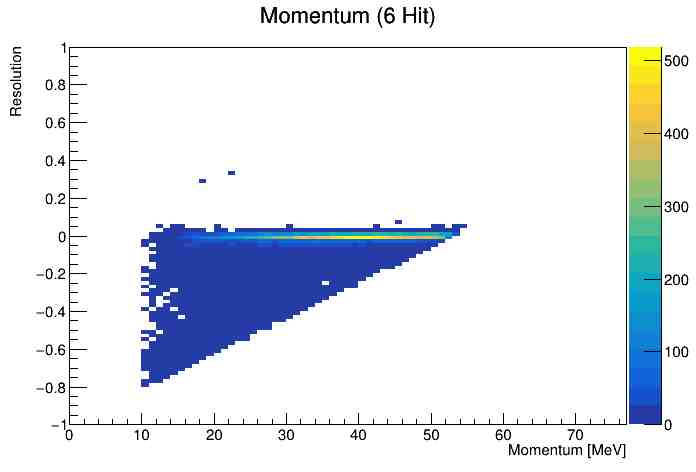
\includegraphics[scale=0.5]{fig/tracking/2dres.jpeg}
    \caption{Figure showing an example of the momentum resolution as a function of measured momentum.}
    \label{fig:resex}
\end{figure}
\par
1-dimensional slices are taken along the x-axis and the associated distributions are fitted with a crystal ball function.
The equation for the crystal ball fit is given below in equation \ref{eq:crysball}.
\begin{equation}
    f(x;\alpha,n,\bar x,\sigma) = N \cdot \begin{cases} \exp(- \frac{(x - \bar x)^2}{2 \sigma^2}), & \mbox{for }\frac{x - \bar x}{\sigma} > -\alpha \\
        A \cdot (B - \frac{x - \bar x}{\sigma})^{-n}, & \mbox{for }\frac{x - \bar x}{\sigma} \leq -\alpha \end{cases}
    \label{eq:crysball}
\end{equation}
From this fitting a mean is taken and an associated error on that mean is also calculated. By iterating this method over each momentum range and for each length of track distributions of the momentum resolutions can be plotted. 
This is shown in figure \ref{fig:resalt}. 
\begin{figure}
    \centering
    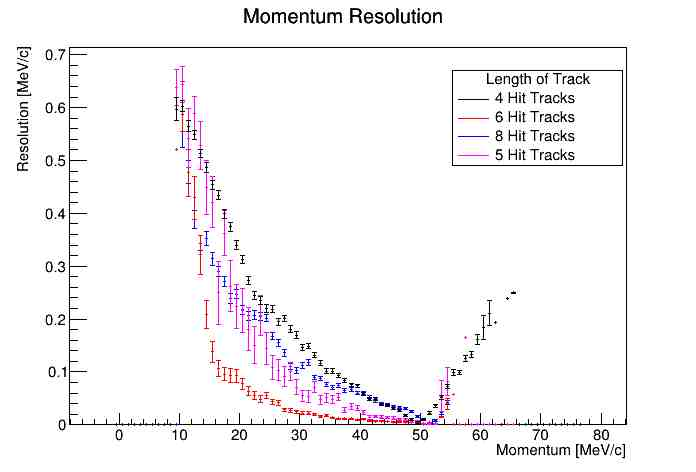
\includegraphics[scale=0.5]{fig/tracking/total_res_alt.jpeg}
    \caption{Figure showing an example of the momentum resolution as a function of measured momentum.}
    \label{fig:resalt}
\end{figure}
\section{Effect of Alternative Tracking}
\textbf{
    \begin{itemize}
        \item This should show the plots of hit efficiency and reconstruction efficiency.
        \item Discuss the difference between layers and why each layer responds differently.
        \item Should also include the effect on vertex reconstruction.
    \end{itemize}
}
\begin{figure}
    \centering
    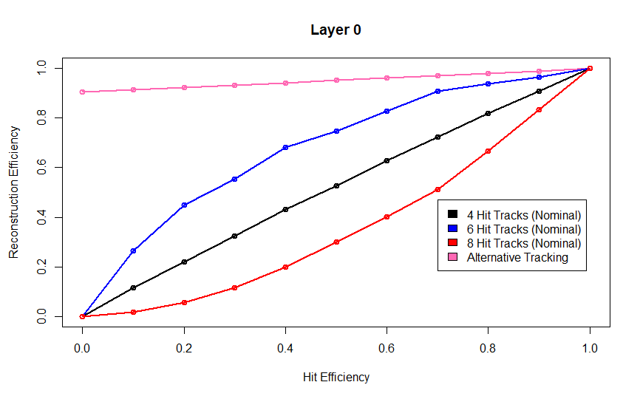
\includegraphics[scale=0.5]{fig/tracking/test_eff.png}
    \caption{Go figure.}
    \label{fig:eff5}
\end{figure}
\begin{figure}
    \centering
    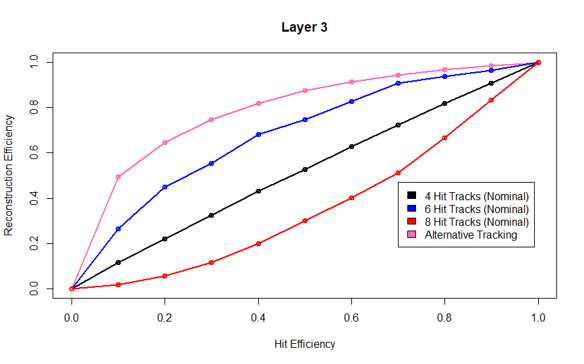
\includegraphics[scale=0.5]{fig/tracking/test_eff3.png}
    \caption{Go figure.}
    \label{fig:eff3}
\end{figure}

	%---------------------------------------------------
	\part{Extra}
	%Extra material here
	%---------------------------------------------------
	%\newpage
	%\printglossary[type=\acronymtype, nonumberlist]
	\newpage
	\begin{appendices}
	Appendix one
	%\input{./chp/app_two.tex}
	\end{appendices}	
	\bibliographystyle{unsrt}
	\bibliography{./chp/ref}
	%---------------------------------------------------
\end{document}